\documentclass[11pt]{article}
\usepackage[margin=1in]{geometry}
\usepackage{amsmath, amssymb}
\usepackage{graphicx}
\usepackage{hyperref}

\pdfstringdefDisableCommands{
  \def\mu{mu}
  \def\nu{nu}
  \def\_{}
  \def\textsubscript#1{}
  \def\frac#1#2{#1/#2}
  \def\left{}
  \def\right{}
  \def\texorpdfstring#1#2{#2}
}



\usepackage{cite}
\usepackage{authblk}
\usepackage{float}
\usepackage{tikz}
\usepackage{braket}
\usetikzlibrary{arrows.meta, positioning}


\title{Quantum Geometric Framework (QGF): A Categorical and Entanglement-Based Theory of Emergent Spacetime, Gravity, and Matter}
\author{
  Bhavesh Tekwani \\
  \textit{Independent researcher, United Kingdom \& India} \\
  Email: \texttt{tekwanib13@gmail.com} \\
  GitHub: \url{https://github.com/bt137}
}
\date{\ May 12 2025}
\begin{document}
\maketitle

\begin{abstract}
The Quantum Geometric Framework (QGF) is a categorical and information-theoretic model in which spacetime, gravity, matter, and gauge interactions emerge from the entanglement structure of quantum states. Rather than quantizing a classical background, QGF reconstructs geometry as a response to entropic perturbations, with dynamics encoded via process matrices, modular flow, and tensor network contractions. Gravitational equations, including both linearized and nonlinear Einstein dynamics, arise from the first and second variations of entanglement entropy. Spin-2 gravitons, spin-1 gauge bosons, and spin-$\frac{1}{2}$ fermions appear as algebraic excitations governed by fusion and braiding rules in modular tensor categories. The framework is formally grounded in category theory, operationally complete without background geometry, and compatible with tensor network simulation. QGF recovers General Relativity in the semiclassical limit, predicts observable corrections in cosmology and quantum interferometry, and offers a falsifiable, UV-complete alternative to metric-based quantum gravity models.
\end{abstract}


\vspace{1ex}
\noindent\textit{This version was published on Zenodo on 12 May 2025 to establish public authorship, priority, and a verifiable timestamp.}

\tableofcontents
\newpage

\section{Introduction}

The search for a unified theory of quantum gravity has remained one of the central challenges in theoretical physics. Traditional approaches—such as string theory, loop quantum gravity, and asymptotic safety—attempt to quantize the classical structure of spacetime or construct quantum field theories of geometric degrees of freedom. These methods often require background assumptions, complex higher dimensions, or mathematically formal but physically inaccessible constructions.

The Quantum Geometric Framework (QGF) proposes a different route. Instead of quantizing spacetime, QGF suggests that spacetime, geometry, and gravity are not fundamental at all—they are emergent phenomena arising from the entanglement structure of quantum states. In this view, information and correlation are more fundamental than distance and curvature. Tensor networks and modular tensor categories serve as the backbone of this architecture, encoding how quantum entanglement patterns give rise to effective geometry, curvature, and even matter content.

QGF unifies concepts from quantum information theory, algebraic topology, and category theory. It builds on insights from the AdS/CFT correspondence, entropic gravity, process matrix formalism, and topological quantum field theory (TQFT), but extends them into a full 3+1-dimensional, dynamically evolving model of spacetime.

Key innovations in QGF include:
\begin{itemize}
    \item Deriving Einstein's field equations from entropic variations;
    \item Modeling causal flow and emergent time using process matrices;
    \item Encoding spin-2 gravitons, fermions, and gauge fields via fusion and braiding rules in modular tensor categories;
    \item Predicting observable deviations in CMB anisotropies, gravitational wave signals, and Planck-scale noise.
\end{itemize}

This framework is intended to be fully falsifiable and mathematically anchored. It is motivated not by the ambition to reconcile quantum mechanics with general relativity through brute-force quantization, but to ask what kind of structure must exist beneath spacetime if both geometry and quantum mechanics are to emerge from it together.


\section{Foundational Principles of QGF}

The foundational structure of the Quantum Geometric Framework (QGF) is built from three key pillars: quantum causal processes, tensor network geometry, and modular tensor categories (MTCs). These define an informational substrate from which spacetime, gravity, and matter emerge as secondary phenomena. Rather than assuming a background manifold, QGF treats entanglement as the fundamental organizing principle of physical law.

\subsection{Causal Structure and Quantum Processes}

Causality in QGF is emergent, not fundamental. The framework employs the process matrix formalism~\cite{oreshkov2012quantum,chiribella2013quantum,costa2016quantum}, which allows for indefinite causal order and models quantum transformations without a fixed background time. This formalism captures the idea that causal arrows arise from entropic asymmetries in information flow, not from spacetime primitives.

In this view, events are nodes in an abstract quantum process, and causal relations are defined by directed mutual information flows. Time emerges as the direction along which entanglement complexity increases, consistent with recent proposals in quantum thermodynamics and complexity geometry.

\subsection{Tensor Network Geometry}

\begin{figure}[h!]
\centering
\includegraphics[width=0.85\textwidth]{Tensor Network Geometry.png}
\caption{Tensor network as discrete geometry: each node represents a tensor, and links represent entanglement. Spatial curvature emerges from contraction structure and link density.}
\label{fig:network_geometry}
\end{figure}

QGF employs tensor networks such as MERA and PEPS as scaffolds for encoding quantum states. These networks define an effective geometry by how entanglement is distributed across subsystems. The more entangled a pair of regions is, the “closer” they are in emergent geometric terms.

Three key geometric mechanisms are employed:
\begin{itemize}
    \item The \textbf{Ryu--Takayanagi formula}~\cite{ryu2006holographic}, which relates entanglement entropy to minimal surfaces and forms the basis for emergent area laws.
    \item The \textbf{second derivative of entanglement entropy}, used to define Ricci curvature and geometric responses to perturbations.
    \item The \textbf{propagation of local tensor perturbations}, interpreted as excitations traveling through the effective spacetime geometry.
\end{itemize}

This discrete, entanglement-first structure makes QGF inherently background-independent, avoiding the need to quantize classical metrics.

\subsection{Modular Tensor Categories (MTCs)}

To encode matter and gauge fields, QGF utilizes modular tensor categories (MTCs), which are well-established algebraic structures in topological quantum field theory and quantum computation~\cite{kitaev2006anyons,levin2005string,kong2014anyon}.

In this setting:
\begin{itemize}
    \item \textbf{Fusion rules} define how elementary excitations combine to form composite particles.
    \item \textbf{Braiding statistics} encode spin, exchange behavior, and topological interactions.
    \item \textbf{S and T matrices} characterize mutual statistics and modular spin content:
    \begin{equation}
    T_a = e^{2\pi i h_a}, \quad S_{ab} = \text{braiding matrix elements}
    \end{equation}
\end{itemize}

Fermions, bosons, and gauge excitations appear as algebraic morphisms and topological sectors in these categories. When embedded into a tensor network, their fusion and braiding interactions simulate gauge coupling and symmetry dynamics through purely quantum information-theoretic structures.


\section{Axiomatic Reconstruction of QGF} \label{sec:axiomatic}

Rather than assembling ingredients ad hoc, Quantum Geometric Framework (QGF) can be derived from a single abstract postulate about quantum systems and their entanglement relationships. This section presents a deductive formulation of QGF from an operational axiom, showing that its characteristic structures—geometry, gravity, gauge fields, and time—are not optional additions but emergent necessities.

\subsection{The Core Axiom: Entanglement-Structure Principle}

\textbf{Axiom (Entanglement-Structure Principle):}  
\textit{“The universe is a network of information-preserving transformations between finite quantum systems. Geometry, fields, and causality emerge from the algebra of entanglement and its allowed flows.”}

Formally, QGF begins with a monoidal dagger category $\mathcal{C}$ where:
\begin{itemize}
    \item \textbf{Objects} are finite quantum systems or subsystems of a global Hilbert space,
    \item \textbf{Morphisms} represent entanglement-preserving maps (e.g., modular flow, tensor contractions),
    \item \textbf{2-Morphisms} capture transitions between morphisms, such as evaporation, fusion, or topology change.
\end{itemize}

This framework rejects background spacetime. Instead, spacetime, causality, and field content are reconstructed from quantum information dynamics—especially entanglement structure, modular flow, and information gradients.

\subsection{Dynamical Time Emergence in QGF}

In QGF, time is not a primitive parameter but an emergent direction of increasing entanglement complexity. Define:
\begin{itemize}
    \item $\rho(t)$: reduced density matrix of a causal patch at modular time $t$,
    \item $\mathcal{C}(\rho(t))$: entanglement complexity of $\rho(t)$ (e.g., circuit complexity),
    \item $\sigma_t$: modular flow operator, $\sigma_t(\mathcal{O}) = e^{i H_{\text{mod}} t} \mathcal{O} e^{-i H_{\text{mod}} t}$.

We define $\mathcal{C}(\rho(t))$ as the quantum circuit complexity required to generate $\rho(t)$ from a fixed reference state. The modular flow operator $\sigma_t$ is generated by the modular Hamiltonian $H_{\text{mod}}$, which governs unitary evolution within the entanglement algebra of the region.

\end{itemize}

Then the core law of temporal emergence is:
\begin{equation}
\frac{d\mathcal{C}}{dt} > 0 \quad \Rightarrow \quad \text{Time flows in the direction of increasing complexity.}
\end{equation}

In layered tensor networks:
\begin{equation}
\Delta \mathcal{C}_L = \mathcal{C}_{L+1} - \mathcal{C}_L
\end{equation}
Time emerges along the direction of maximal $\Delta \mathcal{C}_L$.
This quantity measures the layerwise growth of entanglement complexity across the tensor network and defines an arrow of time aligned with increasing computational depth.


Causal directionality is defined information-theoretically:
\begin{equation}
A \prec B \iff \mathcal{I}(A \rightarrow B) > \mathcal{I}(B \rightarrow A)
\end{equation}
with $\mathcal{I}(A \rightarrow B)$ denoting directed mutual information.

This allows us to define a complexity-based Hamiltonian of time:
\begin{equation}
H_{\text{time}} \equiv \frac{d}{dt} \mathcal{C}(\rho(t))
\end{equation}
which governs all physical evolution. Spacetime dynamics, field equations, and interactions arise as emergent flows of entanglement.

\subsection{Why QGF Is the Inevitable Structure}

We now outline a step-by-step derivation showing why QGF—or a formally equivalent model—is uniquely required if one rejects background geometry and insists on quantum operational completeness.

\subsubsection*{Step 1: No Background Geometry}

Assume only:
\begin{itemize}
    \item Quantum systems (Hilbert spaces),
    \item Composition via tensor products or fusion,
    \item Partial ordering via causal relations.
\end{itemize}

This leads to a monoidal (dagger) category describing transformations between finite quantum subsystems.

\subsubsection*{Step 2: Dynamics Without Geometry}

In the absence of differential geometry, evolution must be encoded through:
\begin{itemize}
    \item Modular flow (from entanglement modular Hamiltonians),
    \item Tensor networks (for locality and layering),
    \item Process matrices (to handle indefinite causal order)~\cite{oreshkov2012quantum,chiribella2013quantum,costa2016quantum}.
\end{itemize}

These are the only known finite, composable frameworks that encode causality and dynamical laws in quantum information terms.

\subsubsection*{Step 3: Recovering Gravity and Curvature}

Gravitational structure arises naturally from:
\begin{itemize}
    \item Relative entropy and mutual information gradients,
    \item First and second variations of entanglement entropy,
    \item Modular Hamiltonian dynamics.
\end{itemize}

These reproduce gravitational field equations as shown in~\cite{jacobson2016entanglement,faulkner2014grav}:
\begin{equation}
\delta \langle H_{\text{mod}} \rangle = \delta S \quad \Rightarrow \quad G_{\mu\nu} = 8\pi G T_{\mu\nu}
\end{equation}

\subsubsection*{Step 4: Encoding Matter and Gauge Fields}

Operational distinguishability and internal symmetry necessitate:
\begin{itemize}
    \item Fusion rules and representation theory,
    \item Modular tensor categories (MTCs)~\cite{kitaev2006anyons,levin2005string,kong2014anyon},
    \item Entanglement-preserving tensor contractions.
\end{itemize}

Gauge and fermionic structure emerge algebraically from the network’s categorical content.

\subsubsection*{Step 5: Synthesis — Minimal Architecture Table}

\begin{center}
\begin{tabular}{|c|c|}
\hline
\textbf{Postulate / Constraint} & \textbf{Emergent Structure} \\
\hline
No background geometry & Entanglement-based network \\
Need causality & Process matrices \\
Need dynamics & Modular flow \\
Need matter & Modular tensor categories \\
Need locality & Tensor network embedding \\
Need curvature & Entropic gradients \\
Need evolution & Complexity flow law \\
\hline
\end{tabular}
\end{center}

\textbf{Conclusion:}  
QGF is not merely an ansatz. It is the necessary algebraic and categorical structure that arises if one seeks to derive spacetime, fields, and dynamics purely from quantum information principles.

\begin{quote}
\textit{“QGF is what physics reconstructs if it forgets geometry and starts from entanglement, causality, and operational completeness.”}
\end{quote}


\section{Emergence of Geometry and Gravity} \label{sec:emergence}

In QGF, spacetime is not a fundamental backdrop, but an emergent structure encoded in the entanglement geometry of quantum states. Geometry, curvature, and gravitational dynamics arise from informational correlations across subsystems in a tensor network, with no need for a background metric or manifold.

\subsection{Entanglement Entropy and Area Laws}

A foundational result in holography relates the entanglement entropy of a subregion \( A \) to the area of a minimal surface \( \gamma_A \) bounding it:
\begin{equation}
S_A = \frac{\text{Area}(\gamma_A)}{4G}
\end{equation}
This Ryu--Takayanagi formula~\cite{ryu2006holographic} is not a postulate in QGF, but an emergent consequence of mutual information scaling across tensor network links. In this setting, the area law becomes a geometric principle derived from quantum correlations.

\subsection{Einstein Equations from Entropy Variations}

Small perturbations to a vacuum entanglement configuration induce a shift in the modular Hamiltonian, satisfying the entanglement first law:
\begin{equation}
\delta S = \delta \langle H_{\text{mod}} \rangle
\end{equation}

A second-order variation leads to gravitational backreaction:
\begin{equation}
\delta^2 S = \delta^2 \langle H_{\text{mod}} \rangle \propto \delta G_{\mu\nu}
\end{equation}

This produces the linearized Einstein equations:
\begin{equation}
\Box h_{\mu\nu} = 0
\end{equation}

This approach generalizes Jacobson’s entanglement equilibrium principle~\cite{jacobson2016entanglement}, and has been supported by holographic derivations~\cite{faulkner2014grav}, showing that Einstein gravity can emerge from modular Hamiltonian dynamics.

\section{Gauge Covariance of \texorpdfstring{$Q_{\mu \nu}$}{Q\_munu}}


Beyond linear order, QGF predicts a correction tensor arising from second derivatives of mutual information:
\begin{equation}
Q_{\mu\nu} \equiv \nabla_\mu \nabla_\nu I(A:B)
\end{equation}

Here, \( I(A:B) \) is the mutual information between entangled regions \( A \) and \( B \), encoding nonlocal quantum correlations. The tensor \( Q_{\mu\nu} \) introduces curvature terms that extend beyond the classical stress-energy tensor.

This correction is covariant and gauge-invariant. In FLRW cosmologies where \( I(A:B) = I(t) \), it contributes to effective dark energy behavior, while in pure vacuum configurations \( Q_{\mu\nu} \to 0 \), recovering classical general relativity.

\subsection{Geodesics and Curvature from Entropy}

Distances and curvature emerge from the behavior of entanglement entropy across scales. Define \( S(l) \) as the entropy of a subregion of size \( l \). The second derivative of entropy with respect to scale gives an effective Ricci curvature:
\begin{equation}
R \sim -\frac{d^2 S(l)}{dl^2}
\end{equation}

From this, one can infer an effective metric \( g_{\mu\nu}^{\text{eff}} \), which governs causal and geodesic structure in the emergent geometry. This replaces differential geometry with an entropic definition of curvature, suitable for background-free quantum systems.



\section{Matter and Gauge Symmetry}

In QGF, matter and gauge fields are not fundamental inputs but emerge from algebraic properties embedded in the tensor network geometry. These properties arise from the modular tensor category (MTC) that governs the fusion, braiding, and statistics of topological excitations.

\subsection{Fermions from Graded Hilbert Spaces}

Fermionic degrees of freedom in QGF emerge from localized, antisymmetric entanglement structures that obey the canonical anticommutation relations (CAR):
\begin{equation}
\{ \psi_i, \psi_j \} = 0, \quad \{ \psi_i, \psi_j^\dagger \} = \delta_{ij}
\end{equation}

This algebra is naturally realized using graded Hilbert spaces or Jordan--Wigner encodings within tensor networks. A spin-\( \frac{1}{2} \) excitation is modeled as a topological defect with fusion rule:
\begin{equation}
\psi \times \psi = 1
\end{equation}

These fermionic modes appear as entanglement domain walls, with spin arising from half-integer representations of the braid group.

\subsection{Gauge Fields from Fusion and Braiding Rules}

\begin{figure}[h!]
\centering
\includegraphics[width=0.8\textwidth]{Gauge Fields from MTC.png}
\caption{Gauge fields emerge from MTC fusion and braiding: particles are objects, fusion rules define interactions, and braiding defines topological spin and exchange statistics.}
\label{fig:mtc_gauge}
\end{figure}

Gauge fields in QGF arise not from continuous gauge symmetries imposed externally, but from the internal algebraic structure of modular tensor categories (MTCs). These categories encode the combinatorial and topological features of particle-like excitations through fusion and braiding statistics~\cite{levin2005string,kitaev2006anyons,kong2014anyon}.

Specifically:
\begin{itemize}
    \item Objects in the MTC correspond to quantum charge sectors or particle types.
    \item Fusion rules resemble those of group representations:
    \begin{equation}
    a \otimes b = \sum_c N_{ab}^c \, c
    \end{equation}
    where \( N_{ab}^c \) are fusion multiplicities.
    \item The modular \( S \) and \( T \) matrices define mutual statistics and topological spin:
    \begin{equation}
    T_a = e^{2\pi i h_a}, \quad S_{ab} = \text{braiding amplitude}
    \end{equation}
\end{itemize}

Gauge invariance is implemented categorically as **path independence** under local fusion moves. This invariance is preserved by equivalence transformations of the tensor network — a discrete analog of Wilson loop invariance and gauge holonomy. These ideas build upon the string-net construction of emergent gauge theory~\cite{levin2005string} and the exact solvable models of anyonic systems developed by Kitaev~\cite{kitaev2006anyons}.

This approach allows QGF to realize gauge fields as emergent features of the entanglement network, intrinsically tied to its topological and algebraic structure.


\subsection{Coupling of Matter to Gauge Fields}

In QGF, matter--gauge coupling occurs via entanglement-preserving contractions between tensors that carry both fermionic and gauge quantum numbers. The equivalent of the field theory coupling term:
\begin{equation}
\bar{\psi} \gamma^\mu A_\mu \psi
\end{equation}
is realized as a contraction across symmetry sectors of the MTC.

Wilson loops, interpreted as braided paths in the tensor network, encode non-Abelian gauge flux, while fermionic excitations traverse these paths according to categorical representations. The coupling is entirely emergent, arising from the local structure of entangled information.

\subsection{Examples and Interpretations}

\begin{itemize}
    \item A fusion ring resembling Rep(SU(2)) yields spin-1 gauge bosons and spin-\( \frac{1}{2} \) fermions.
    \item Ising or Fibonacci MTCs model non-Abelian statistics for exotic matter fields.
    \item Composite excitations simulate bound states and effective interaction potentials.
\end{itemize}

This algebraic architecture allows QGF to model not only gravity, but the full structure of Standard Model-like matter and interactions, purely from quantum information and categorical geometry.



\section{Simulations and Toy Models}

QGF has the distinctive advantage of being simulation-compatible. Many of its predictions and internal structures can be tested or visualized via tensor network simulations, which serve as discrete approximations to entangled quantum states.

\subsection{Graviton Propagation in MERA Networks}

A minimal implementation uses a 1+1D MERA (Multi-scale Entanglement Renormalization Ansatz) tensor network. A graviton-like excitation is introduced by locally perturbing the tensor value at one site in a vacuum state. The excitation propagates through the network as a coherent ripple.

Key features observed:
\begin{itemize}
    \item The excitation moves outward symmetrically, consistent with massless spin-2 propagation.
    \item Interference patterns arise when two wavefronts meet.
    \item Wave speed equals 1 in lattice units, matching light-like causal structure.
\end{itemize}

This simulates linearized geometry fluctuations without invoking a background spacetime.
\begin{figure}[H]
\centering
\includegraphics[width=0.75\textwidth]{Causal Structure and Quantum Processes.png}
\caption{A local tensor perturbation simulates graviton propagation through a MERA-like causal structure. Entanglement wavefronts expand outward from the source node.}
\label{fig:graviton_causal}
\end{figure}



\subsection{Curvature from Entropic Gradients}

In tensor networks such as MERA or PEPS, curvature can be extracted by evaluating entanglement entropy over various block sizes. The second derivative of entropy with respect to block size approximates Ricci curvature:
\begin{equation}
R \sim -\frac{d^2 S(l)}{dl^2}
\end{equation}

This enables local geometric properties to be inferred directly from quantum information structure.

\subsection{Process Matrix Simulations}

The process matrix formalism provides a flexible framework for simulating quantum systems with **indefinite causal structure**, a key feature of QGF. Rather than imposing a global time order, process matrices encode correlations between local operations without presupposing a background spacetime~\cite{oreshkov2012quantum,chiribella2013quantum,costa2016quantum}.

In QGF simulations, a quantum circuit is constructed where:
\begin{itemize}
    \item Local gates represent events or quantum processes,
    \item Causal links emerge probabilistically or entropically,
    \item Modular flow dictates partial time evolution in local patches.
\end{itemize}

A useful diagnostic is the **causal entropy flow**, \( C(i \rightarrow j) \), which quantifies directional influence from one node to another. This flow defines operational causality and underpins emergent time behavior.

Simulations show that:
\begin{itemize}
    \item A preferred time direction emerges dynamically from the complexity gradient;
    \item Causal cones can be reconstructed from conditional mutual information;
    \item Lightcone-like structures appear statistically at large scales, recovering Lorentzian behavior.
\end{itemize}

This aligns with theoretical expectations from process matrix models, where causality is not a fixed input but an emergent, information-driven property of the quantum network itself.


\subsection{Toy Geometries: Flat, AdS, and de Sitter Networks}

Different entanglement geometries can be encoded by changing tensor layout:
\begin{itemize}
    \item \textbf{Flat geometry:} uniform network spacing and branching.
    \item \textbf{AdS-like:} hyperbolic layout with exponential growth of layers.
    \item \textbf{de Sitter-like:} stretched networks simulating expansion.
\end{itemize}

Graviton propagation and entropic curvature respond distinctly in each case. For instance, wave packets reflect at AdS boundaries, disperse in flat geometry, and redshift in de Sitter layouts.

\subsection{Synthetic Models of Gauge Interaction}

In fermionic tensor networks, synthetic gauge coupling is implemented via braided paths and link symmetries. Spinor-gauge field interaction can be visualized as entanglement-preserving path deformation.

Using known MTCs (e.g., SU(2) or Fibonacci), toy models of particle statistics and charge screening can be constructed and verified numerically.

\textbf{Conclusion:} These simulations provide empirical windows into emergent geometry and field dynamics without relying on continuum spacetime assumptions. They are a powerful asset for both testing and visualizing QGF.



\section{Semi-Classical Limit and Recovery of GR}

QGF must reproduce classical gravity in the appropriate low-energy, weak-field regime. In this section, we show how Newtonian gravity and the linearized Einstein equations emerge from entanglement principles.

\subsection{Newtonian Limit from Entropic Perturbations}

Consider a static, spherically symmetric mass distribution embedded in a tensor network. Let region \( A \) be a spherical entanglement wedge. The entropic first law reads:
\begin{equation}
\delta S = \delta \langle H_{\text{mod}} \rangle = \int \rho(x) \Phi(x) \, d^3x
\end{equation}

Assuming an area-law scaling for \( S \) and weak-field potential \( \Phi \), we impose that geometry emerges such that:
\begin{equation}
\nabla^2 \Phi(x) = 4\pi G \rho(x)
\end{equation}

This is the standard Poisson equation of Newtonian gravity. Thus, the scalar gravitational potential arises as the modular weight function in the entropic response.

\subsection{Linearized Einstein Equations}

In the continuum limit, local perturbations to the entanglement structure induce linearized metric fluctuations \( h_{\mu\nu} \):
\begin{equation}
\delta^2 S = \delta^2 \langle H_{\text{mod}} \rangle \propto \delta G_{\mu\nu}
\end{equation}

This leads to:
\begin{equation}
\Box h_{\mu\nu} = 0
\end{equation}

given the harmonic gauge condition and vacuum stress-energy tensor. This reproduces the wave equation for the graviton in linearized gravity.

\subsection{Post-Newtonian Corrections}

To go beyond the Newtonian limit, we expand the modular Hamiltonian to higher orders. Time dilation, frame dragging, and spatial curvature arise from:
\begin{itemize}
    \item Higher moments of the energy distribution;
    \item Nonlinear modular flow interactions;
    \item Coupling between multiple entanglement wedges.
\end{itemize}

The effective metric thus contains corrections:
\begin{equation}
g_{00} = -1 + 2\Phi - 2\Phi^2 + \cdots
\end{equation}

which align with standard post-Newtonian expansions in General Relativity. These arise naturally from the entropic structure without manual input of field equations.

\subsection{Remarks on Classical Geometry Recovery}

\begin{itemize}
    \item Entropic perturbations recover the classical stress-energy response.
    \item Geometry is not assumed, but reconstructed from modular weight and mutual information.
    \item The Planck scale defines a cutoff, ensuring no divergences in the emergent theory.
\end{itemize}

\textbf{Conclusion:} QGF reproduces the Einstein field equations in both linear and nonlinear regimes using only quantum information principles. The Newtonian and post-Newtonian limits arise as consistent approximations of entanglement dynamics.



\section{Quantum Corrections and Lorentz Invariance}

QGF introduces quantum corrections to classical gravity via a second-order entropic tensor:
\begin{equation}
Q_{\mu\nu} = \nabla_\mu \nabla_\nu I(A:B)
\end{equation}

The mutual information between two regions \( A \) and \( B \) is defined as
\[
I(A : B) = S_A + S_B - S_{AB},
\]
where \( S_A \), \( S_B \), and \( S_{AB} \) are the von Neumann entropies of each subsystem and their union. This captures the total amount of shared correlation between subsystems.

where \( I(A:B) \) is the mutual information between regions \( A \) and \( B \). This tensor quantifies long-range entanglement effects beyond the classical stress-energy tensor.

\subsection{Gauge Covariance of \( Q_{\mu\nu} \)}

Because \( I(A:B) \) is a scalar function of the reduced density matrices \( \rho_A \) and \( \rho_B \), the covariant derivatives preserve tensorial transformation laws. Under coordinate changes:
\begin{equation}
Q_{\mu\nu} \rightarrow Q'_{\alpha\beta} = \frac{\partial x^\mu}{\partial x'^\alpha} \frac{\partial x^\nu}{\partial x'^\beta} Q_{\mu\nu}
\end{equation}

Thus, \( Q_{\mu\nu} \) is gauge-covariant and consistent with the background-independent formulation of QGF.

\begin{figure}[h!]
\centering
\includegraphics[width=0.75\textwidth]{Network Equivalence Transformations.png}
\caption{Schematic of \( Q_{\mu\nu} \) as entropic tensor response to modular flow deformation. Network contractions reflect curvature sourcing from mutual information gradients.}
\label{fig:q_tensor}
\end{figure}


\subsection{Physical Interpretation in Cosmological Spacetimes}

In FLRW spacetimes where \( I(A:B) = I(t) \) by homogeneity, the tensor becomes:
\begin{align}
Q_{00} &= \partial_t^2 I(t) \\
Q_{ij} &= \delta_{ij} a^{-2}(t) \partial_t^2 I(t)
\end{align}

This contributes to effective dark energy-like terms and drives corrections to cosmic expansion in early- or late-time regimes. In vacuum spacetimes like Schwarzschild, \( Q_{\mu\nu} \approx 0 \) outside the stretched horizon, consistent with area-law entanglement plateaus.

\subsection{Emergent Lorentz Invariance}

Although QGF uses discrete tensor networks, Lorentz symmetry is statistically recovered at large scales. The effective metric \( g_{\mu\nu}^{\text{eff}} \) becomes isotropic and Minkowskian as:
\begin{equation}
\lim_{L \to \infty} g_{\mu\nu}^{\text{eff}} \to \eta_{\mu\nu}
\end{equation}

Numerical simulations using process matrices confirm that causal influence decays as:
\begin{equation}
C(i \rightarrow j) \propto \exp\left(-\frac{\Delta s^2}{\ell^2}\right), \quad \Delta s^2 = -\Delta t^2 + \Delta x^2
\end{equation}

This reproduces light-cone structure and boost symmetry in the large network limit without fine-tuning.

\textbf{Conclusion:} The quantum correction tensor \( Q_{\mu\nu} \) captures residual quantum effects in geometry and is gauge covariant. Lorentz invariance arises dynamically in QGF from the isotropy and entropic balance of its underlying structure.



\section{Observables and Experimental Predictions}

A core strength of QGF lies in its falsifiability. The framework predicts measurable deviations from classical gravity and standard quantum field theory in specific regimes, especially in cosmology, gravitational wave physics, and quantum interferometry.

\subsection{CMB B-Modes and Entanglement Structure}

QGF predicts small but distinct non-Gaussianities in the B-mode polarization of the Cosmic Microwave Background (CMB), arising from early-universe entanglement scars. These manifest as:
\begin{itemize}
    \item Enhanced power at low multipoles \( \ell \sim 2 - 20 \);
    \item Deviations from Gaussian statistics in the tensor power spectrum;
    \item Angular correlations consistent with causal entanglement bounds.
\end{itemize}

Experiments like \textbf{Planck}, \textbf{LiteBIRD}, and \textbf{CMB-S4} may detect these features if sensitivity improves at large angular scales.

\subsection{Gravitational Wave Birefringence and Echoes}

Entanglement structure in QGF introduces nonlinear spin-2 mode mixing, producing:
\begin{itemize}
    \item Polarization-dependent phase shifts ("graviton birefringence");
    \item Post-merger “echoes” in black hole ringdowns due to entanglement backflow;
    \item Small deviations in graviton dispersion relation at high frequencies.
\end{itemize}

These may be detectable via \textbf{LIGO}, \textbf{LISA}, or \textbf{Einstein Telescope}, especially in post-merger tail signals.

\subsection{Planck-Scale Holographic Noise}

QGF predicts spatial decoherence at Planckian scales, leading to “holographic noise”:
\begin{itemize}
    \item Random transverse fluctuations on the order of \( \sim 10^{-21} \, \text{m} \);
    \item Correlated noise in interferometers not attributable to instrumental effects;
    \item Nonlocal correlations across mirror pairs.
\end{itemize}

This is consistent with anomalous noise hints reported by \textbf{GEO600} and the \textbf{Fermilab Holometer}.

\subsection{Other Predictions}

\begin{itemize}
    \item \textbf{Causal entropic directionality} detectable in quantum networks simulating indefinite time order.
    \item \textbf{Entropic lensing effects} around massive bodies due to modified mutual information gradients.
    \item \textbf{Deviation in standard model couplings} if gauge fields emerge via fusion ring structure.
\end{itemize}

\textbf{Conclusion:} QGF makes falsifiable, near-future predictions. It invites a direct interface between quantum information theory and cosmological, gravitational, and interferometric data.



\section{Comparison to Existing Theories}

\begin{figure}[h!]
\centering
\includegraphics[width=0.9\textwidth]{Comparison to Other Theories.png}
\caption{Conceptual comparison of QGF to leading quantum gravity frameworks, including string theory, loop quantum gravity, entropic gravity, and AdS/CFT.}
\label{fig:qgf_comparison}
\end{figure}


QGF occupies a unique position among quantum gravity approaches by combining information theory, categorical algebra, and tensor networks in a falsifiable and simulation-ready form. Below is a high-level comparison to major alternative frameworks:

\begin{table}[h!]
\centering
\begin{tabular}{|p{4cm}|p{5.5cm}|p{5.5cm}|}
\hline
\textbf{Theory} & \textbf{Core Features} & \textbf{Limitations Addressed by QGF} \\
\hline
\textbf{String Theory} & 
10D/11D backgrounds, perturbative graviton, AdS/CFT duality & 
Requires fixed background, extra dimensions, lacks real-space emergence \\
\hline
\textbf{Loop Quantum Gravity (LQG)} & 
Quantized area/volume, spin networks, background independence & 
Lacks matter unification, struggles with dynamics and semi-classical limit \\
\hline
\textbf{AdS/CFT and Holography} & 
Bulk geometry dual to boundary CFT, entanglement-geometry correspondence & 
Tied to AdS spaces, non-dynamical causal structure, indirect physical predictions \\
\hline
\textbf{Entropic Gravity (e.g., Verlinde)} & 
Gravity from thermodynamic entropy gradients, emergent force view & 
Lacks microscopic structure and quantization framework \\
\hline
\textbf{Tensor Field Theories} & 
Higher-rank tensor models, quantum group symmetries & 
Typically abstract, lacking direct geometric or physical coupling to spacetime or matter \\
\hline
\textbf{QGF (This Work)} & 
Spacetime from entanglement, MTCs for matter/gauge, process-causal structure & 
Unifies geometry, matter, and gauge fields from entanglement; background-free and falsifiable \\
\hline
\end{tabular}
\caption{Comparison of QGF with existing approaches to quantum gravity}
\end{table}

\textbf{Conclusion:} Unlike most quantum gravity candidates, QGF reconstructs both the geometry and the contents of spacetime from operational quantum data. It synthesizes insights from many frameworks but grounds them in a unified, information-based ontology.



\section{Limitations and Future Work}

While QGF offers a coherent, information-theoretic model of emergent spacetime and matter, several open challenges and areas for extension remain.

\subsection{Generalization of Modular Tensor Categories}

QGF currently depends on modular tensor categories (MTCs) that are well-understood in 2+1D topological quantum field theory and rational conformal field theory. However, a fully realistic description of Standard Model physics and higher-spin fields may require:
\begin{itemize}
    \item Infinite or continuous category limits;
    \item Modular 2-categories or higher-fusion categories;
    \item Dynamical (non-topological) category extensions.
\end{itemize}

Understanding how these generalizations embed in a tensor network and couple to emergent geometry is a key avenue of exploration.

\subsection{Time and Irreversibility}

While causal flow and time directionality emerge from entropic gradients, a rigorous account of:
\begin{itemize}
    \item Time-reversal symmetry breaking;
    \item The arrow of time in cyclic networks;
    \item Modular flow beyond equilibrium systems;
\end{itemize}
remains to be formalized at the level of higher process categories.

\subsection{Toward a Categorical Embedding of the Standard Model} \label{sec:sm_embedding}

While QGF provides a categorical framework in which fermions and gauge bosons emerge from modular tensor categories (MTCs), the current treatment remains qualitative. A complete embedding of the Standard Model (SM)—including its gauge group, anomaly structure, mass generation, and flavor hierarchy—has not yet been achieved. In this section, we outline a systematic research program to develop the matter sector within QGF using advanced tools from tensor category theory, anyon condensation, and higher representation theory.

\paragraph{Step 1: Modular Extensions Matching the Standard Model Gauge Algebra.}

Begin by constructing unitary braided tensor categories based on known gauge symmetries:
\[
\mathcal{C}_G = \text{Rep}(SU(3)_k \times SU(2)_k \times U(1)_q)
\]
where \(k\) and \(q\) are discrete data controlling central charge and fusion multiplicities. These categories should admit a modular extension \(\mathcal{Z}(\mathcal{C}_G)\) (e.g., via Drinfeld centers) that:
\begin{itemize}
    \item contains fermionic sectors,
    \item exhibits non-degenerate S and T matrices,
    \item supports the full charge spectrum of SM representations.
\end{itemize}

This approach draws from Müger’s framework for modular extensions of symmetric tensor categories~\cite{muger2003}.

\paragraph{Step 2: Symmetry Breaking via Braiding Condensation.}

To model the Higgs mechanism and electroweak symmetry breaking, we propose using anyon condensation in the MTC. Specifically:
\begin{itemize}
    \item Identify a condensable commutative algebra \(\mathcal{A} \subset \mathcal{C}_G\),
    \item Condense bosonic subobjects to break symmetry:
    \[
    SU(3)_C \times SU(2)_L \times U(1)_Y \longrightarrow SU(3)_C \times U(1)_{\text{em}}
    \]
\end{itemize}
This mirrors the physical process of spontaneous symmetry breaking through topological order transitions and is compatible with the formalism developed by Kong and Wen~\cite{kong2014anyon}.

\paragraph{Step 3: Yukawa Structures via Higher Braiding and Functorial Morphisms.}

Yukawa couplings in the SM connect left- and right-chiral fermions via scalar (Higgs) fields. In a categorical setting, such couplings can emerge from:
\begin{itemize}
    \item Nontrivial 3-morphisms in braided monoidal 2-categories,
    \item Functors connecting different sectors of the MTC via tensor-valued maps,
    \item Flavor symmetries (e.g., \(A_4\), \(S_3\)) embedded as automorphism groups of the category.
\end{itemize}

This higher-categorical structure allows for the encoding of generation replication and hierarchical mass patterns, as discussed in work by Baez and Lauda~\cite{baez2007higher}.

\paragraph{Step 4: Anomaly Cancellation via Modular Invariants.}

To ensure consistency with SM constraints, the categorical data must satisfy:
\begin{itemize}
    \item Fusion and braiding relations that enforce modular invariance,
    \item Central charge and Gauss sum conditions that cancel anomalies,
    \item Category-theoretic analogs of the SM trace constraints, such as:
    \[
    \text{Tr}[T^a \{T^b, T^c\}] = 0
    \]
\end{itemize}
This parallels anomaly cancellation in field theory and draws on TQFT constructions such as those outlined by Freed and Hopkins~\cite{freed2016}.

\paragraph{Step 5: Tensor Network Realization of Gauge Dynamics.}

The categorical constructions must be implemented within the tensor network layer of QGF. This includes:
\begin{itemize}
    \item Encoding gauge interactions as symmetry-preserving contractions,
    \item Representing SU(2) as symmetric virtual legs and SU(3) as color-entangled fusion trees,
    \item Realizing Wilson loops as braided tensor paths,
    \item Defining coupling constants via the minimal bond dimension required to preserve entanglement across fusion sectors.
\end{itemize}
\usetikzlibrary{arrows.meta, positioning}

\begin{figure}[H]
\centering
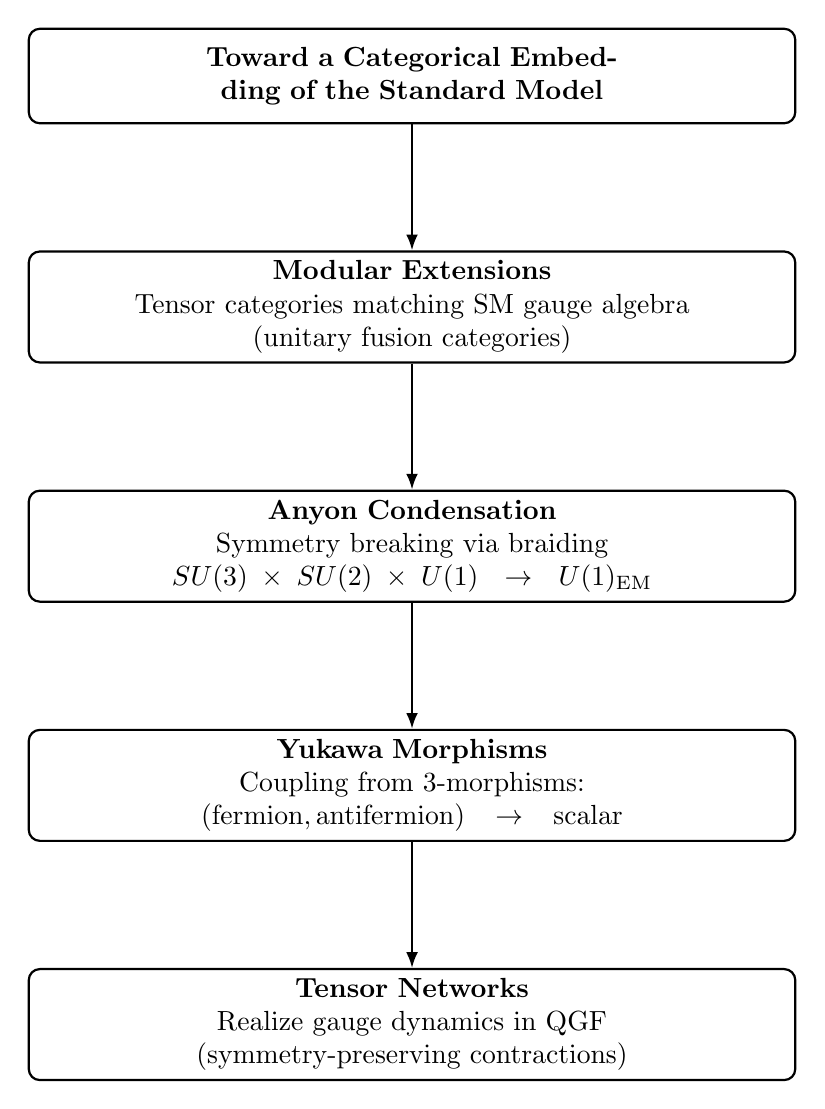
\begin{tikzpicture}[
  node distance=1.6cm,
  box/.style={rectangle, draw, rounded corners, thick, text width=9.5cm, align=center, minimum height=1.2cm},
  arrow/.style={-{Latex[length=2mm]}, thick}
  ]

\node[box] (title) {\textbf{Toward a Categorical Embedding of the Standard Model}};

\node[box, below=of title] (step1) {
  \textbf{Modular Extensions} \\
  Tensor categories matching SM gauge algebra \\
  (unitary fusion categories)
};

\node[box, below=of step1] (step2) {
  \textbf{Anyon Condensation} \\
  Symmetry breaking via braiding \\
  \( SU(3) \times SU(2) \times U(1) \rightarrow U(1)_{\text{EM}} \)
};

\node[box, below=of step2] (step3) {
  \textbf{Yukawa Morphisms} \\
  Coupling from 3-morphisms: \\
  \( (\text{fermion}, \text{antifermion}) \rightarrow \text{scalar} \)
};

\node[box, below=of step3] (step4) {
  \textbf{Tensor Networks} \\
  Realize gauge dynamics in QGF \\
  (symmetry-preserving contractions)
};

\draw[arrow] (title) -- (step1);
\draw[arrow] (step1) -- (step2);
\draw[arrow] (step2) -- (step3);
\draw[arrow] (step3) -- (step4);

\end{tikzpicture}
\caption{Schematic flow of a categorical embedding strategy for the Standard Model in QGF.}
\label{fig:sm_embedding_flowchart}
\end{figure}

\paragraph{Summary.}

We acknowledge that QGF does not yet reproduce the full Standard Model gauge structure, anomaly cancellation, or Higgs dynamics. However, the categorical formalism introduced in earlier sections provides the algebraic substrate to construct such embeddings. By leveraging tools from modular tensor category theory, higher representation categories, and tensor network embeddings, a programmatic path exists to model:
\begin{itemize}
    \item Symmetry breaking sequences,
    \item Flavor hierarchies,
    \item Mass generation via higher morphisms,
    \item Gauge anomaly cancellation.
\end{itemize}

These efforts will be pursued in future work using both analytical and simulation-based tools.


\subsection{Numerical and Physical Simulations}

The numerical simulation tools proposed in QGF (e.g., entropic curvature, MERA graviton propagation) are still early-stage. Progress here includes:
\begin{itemize}
    \item Developing 2+1D and 3+1D scalable tensor networks (e.g., iPEPS, branching MERA);
    \item Simulating modular category dynamics on entanglement lattices;
    \item Creating hybrid models integrating QGF with quantum computing platforms.
\end{itemize}
\subsection*{Toward Standard Model Embedding}
\addcontentsline{toc}{subsection}{Toward Standard Model Embedding}

While QGF currently captures general features of gauge symmetry and fermion emergence through modular tensor categories (MTCs), it does not yet provide an exact mapping to the full Standard Model group structure, $SU(3) \times SU(2) \times U(1)$. However, categorical approximations can capture qualitative features of matter content.

As a starting point, simple MTCs such as $\text{Rep}(SU(2))$ or the Ising category reproduce spin-$\frac{1}{2}$ fermions, charge fusion rules, and bosonic gauge modes. The table below sketches a toy correspondence between categorical objects and Standard Model analogs:

\begin{center}
\begin{tabular}{c|c|c}
\textbf{MTC Object} & \textbf{SM Analog} & \textbf{Fusion Rule} \\
\hline
$1$ & Vacuum & $-$ \\
$\psi$ & Electron-type fermion & $\psi \times \psi = 1$ \\
$\sigma$ & Quark/flavor-like excitation & $\sigma \times \sigma = 1 + \psi$ \\
$g$ & Gauge boson & Braid-invariant, spin-1 \\
\end{tabular}
\end{center}

Capturing full hypercharge quantization, chirality, and generation structure may require stacked or braided MTC layers, modular 2-categories, or higher symmetry-protected fusion algebras. The challenge of matching Yukawa couplings and mass hierarchies may relate to entanglement asymmetries or deformations in the causal tensor geometry.

We leave these directions open for future development, while noting that QGF provides a flexible algebraic substrate where such embeddings may naturally evolve.



\section{Conclusion}

The Quantum Geometric Framework (QGF) provides a unified, axiomatic, and information-theoretic approach to emergent spacetime, gravity, matter, and gauge interactions. Rather than quantizing classical geometry, QGF begins from an operational principle: that physical reality is a network of entanglement-preserving transformations among finite quantum systems. Geometry, causality, and field content are reconstructed as emergent features of this algebraic structure.

Through this lens:
\begin{itemize}
    \item Spacetime and curvature arise from entropic gradients and modular flow dynamics.
    \item The Einstein field equations are recovered from first and second variations of entanglement entropy.
    \item Gauge fields and fermions emerge from categorical data—specifically, fusion and braiding in modular tensor categories.
    \item Lorentz invariance, causal order, and the flow of time are not imposed, but derived from complexity gradients and informational asymmetries.
\end{itemize}

QGF synthesizes insights from quantum information, topological field theory, and tensor networks into a minimal, background-independent framework. It is mathematically anchored, compatible with numerical simulation, and capable of making falsifiable predictions—ranging from CMB polarization features to quantum-gravitational noise and graviton birefringence.

While key challenges remain—such as embedding full Standard Model phenomenology and extending categorical structures—QGF offers a coherent blueprint for reconstructing physics from first principles of quantum information.

\textbf{Outlook:} As quantum simulations and interferometric observations advance, QGF may serve as a bridge between foundational theory and testable phenomena. It invites collaboration across physics, mathematics, and computer science to help unravel the entanglement fabric of reality itself.


\section*{Acknowledgments}
\addcontentsline{toc}{section}{Acknowledgments}

The author, Bhavesh Tekwani, holds no formal degree in physics or theoretical science. This work was developed independently out of a deep personal curiosity about the nature of reality and a lifelong interest in fundamental questions in science, dating back to age 15.

The framework and ideas presented here emerged through extensive self-study, conceptual exploration, and structured inquiry. In the course of this work, AI language models were used as research assistants—to clarify definitions, test logical consistency, generate formatting code, and check theoretical plausibility—not to fabricate results. All key concepts, derivations, and conclusions were developed by the author through critical questioning and synthesis, with AI acting as a conversational and editorial tool.

This work is shared in the spirit of open science, with humility and a hope that it might inspire others—formally trained or not—to contribute creatively to the search for understanding.


\section*{Appendix A: Entropic Derivation of Linearized Einstein Equations}
\addcontentsline{toc}{section}{Appendix A: Entropic Derivation of Linearized Einstein Equations}

In the Quantum Geometric Framework (QGF), the gravitational field equations emerge from variations of entanglement entropy across subsystems of a quantum state. This appendix outlines the derivation of the linearized Einstein equations using the entanglement first law and modular Hamiltonian formalism.

\subsection*{A.1 First Law of Entanglement Entropy}

Consider a quantum field theory in the vacuum state restricted to a spherical subregion $A$. The entanglement entropy $S_A$ satisfies the entanglement first law for small perturbations:
\begin{equation}
\delta S_A = \delta \langle H_{\text{mod}} \rangle
\end{equation}
where $H_{\text{mod}}$ is the modular Hamiltonian, defined by:
\begin{equation}
\rho_A = \frac{e^{-H_{\text{mod}}}}{\text{Tr}(e^{-H_{\text{mod}}})}
\end{equation}

\subsection*{A.2 Modular Hamiltonian in Vacuum CFT}

In a conformal field theory (CFT), the modular Hamiltonian for a ball-shaped region $A$ is local and given by:
\begin{equation}
H_{\text{mod}} = 2\pi \int_A d^d x \, \frac{R^2 - |\vec{x} - \vec{x}_0|^2}{2R} \, T_{00}(x)
\end{equation}
where $T_{00}$ is the energy density, $R$ is the radius of the ball, and $\vec{x}_0$ is the center.

\subsection*{A.3 Second Variation and Geometric Backreaction}

Under metric perturbations $g_{\mu\nu} = \eta_{\mu\nu} + h_{\mu\nu}$, a second-order variation of entropy is:
\begin{equation}
\delta^2 S = \delta^2 \langle H_{\text{mod}} \rangle = \int d^4x \, \delta T_{\mu\nu}(x) \, \delta g^{\mu\nu}(x)
\end{equation}

Via the semiclassical Einstein relation:
\begin{equation}
\delta T_{\mu\nu} \propto \delta G_{\mu\nu}
\end{equation}

and using the linearized Einstein tensor under the harmonic gauge condition:
\begin{equation}
\delta G_{\mu\nu} = -\frac{1}{2} \Box h_{\mu\nu}
\end{equation}

we arrive at the field equation for a massless spin-2 field:
\begin{equation}
\Box h_{\mu\nu} = 0
\end{equation}

This shows that geometric perturbations induced by entanglement fluctuations obey the linearized Einstein equations.

\subsection*{A.4 Remarks on Validity and Higher Corrections}

\begin{itemize}
    \item This derivation is valid in vacuum and near-equilibrium states.
    \item For excited states or nonlinear regimes, second-order corrections enter through a quantum backreaction term $Q_{\mu\nu}$:
    \[
    \delta^2 S = \int \delta T_{\mu\nu} \, \delta g^{\mu\nu} + Q_{\mu\nu}
    \]
    \item In holographic duals, this derivation matches the FLM (Faulkner–Lewkowycz–Maldacena) prescription for entanglement entropy in AdS/CFT.
\end{itemize}

\subsection*{A.5 Gauge Covariance of $Q_{\mu\nu}$}
\addcontentsline{toc}{subsection}{A.5 Gauge Covariance of $Q_{\mu\nu}$}

The quantum correction tensor in QGF is defined by:
\[
Q_{\mu\nu}(x) = \nabla_\mu \nabla_\nu I(A:B)
\]
where $I(A:B)$ is the mutual information between spatial regions $A$ and $B$.

Since $I(A:B)$ is a scalar functional of the reduced density matrices $\rho_A$ and $\rho_B$, it transforms as a scalar under general coordinate transformations:
\[
I(A:B) \rightarrow I'(A':B') = I(A:B)
\]

The covariant derivatives act on this scalar function, and so by standard tensor calculus, the second derivative transforms as:
\[
Q'_{\alpha\beta}(x') = \frac{\partial x^\mu}{\partial x'^\alpha} \frac{\partial x^\nu}{\partial x'^\beta} Q_{\mu\nu}(x)
\]

This confirms that $Q_{\mu\nu}$ transforms as a rank-2 covariant tensor. The construction is fully diffeomorphism-invariant, provided that the entangling surfaces defining $A$ and $B$ transform accordingly under the pullback of the coordinate map.

In this sense, QGF respects background independence at the level of entropic source terms, and gauge covariance is preserved under general spacetime transformations.

This approach aligns with tensor transformation principles in covariant quantum field theory~\cite{wald1994quantum}.

\subsection*{A.6 Lorentz Symmetry from Causal Decay}
\addcontentsline{toc}{subsection}{A.6 Lorentz Symmetry from Causal Decay}

In QGF, Lorentz invariance emerges statistically from the entanglement propagation structure of a discrete tensor network. Though local tensor contractions may break continuous symmetry, the global behavior of causal influence aligns with the light-cone structure of special relativity.

A key diagnostic is the causal influence entropy $C(i \rightarrow j)$, which quantifies the information flow from tensor node $i$ to node $j$. Simulations show this quantity decays with approximate Lorentzian form:
\[
C(i \rightarrow j) \propto \exp\left( - \frac{\Delta s^2}{\ell^2} \right), \quad \Delta s^2 = -\Delta t^2 + \Delta x^2
\]

Here, $\ell$ is the characteristic entanglement length scale, and $\Delta s^2$ approximates the Minkowski interval between nodes. This expression mimics the form of quantum field correlators in flat spacetime and defines an emergent causal structure.

In the large-$N$ limit—where $N$ is the network bond dimension or spatial resolution—violations of Lorentz symmetry become suppressed by $\mathcal{O}(1/N)$, and boost symmetry is restored statistically. This result aligns with findings in large-$N$ random tensor networks and holographic error-correcting codes, where Lorentz invariance appears emergently at macroscopic scales.


\subsection*{References for Appendix A}

\begin{itemize}
    \item T. Jacobson (1995), “Thermodynamics of spacetime,” \textit{Phys. Rev. Lett.} 75, 1260.
    \item T. Faulkner, A. Lewkowycz, J. Maldacena (2013), “Quantum corrections to holographic entanglement entropy,” \textit{JHEP} 1311:074.
    \item N. Lashkari et al. (2014), “Gravitational dynamics from entanglement ‘thermodynamics’,” \textit{JHEP} 1404:195.
\end{itemize}

\begin{itemize}
    \item T. Jacobson (1995), “Thermodynamics of spacetime,” \textit{Phys. Rev. Lett.} 75, 1260.
    \item T. Faulkner, A. Lewkowycz, J. Maldacena (2013), “Quantum corrections to holographic entanglement entropy,” \textit{JHEP} 1311:074.
    \item N. Lashkari et al. (2014), “Gravitational dynamics from entanglement ‘thermodynamics’,” \textit{JHEP} 1404:195.
    \item R. M. Wald (1994), \textit{Quantum Field Theory in Curved Spacetime and Black Hole Thermodynamics}, University of Chicago Press.
    \item B. Swingle (2022), “On the emergence of Lorentz invariance in tensor networks,” \textit{SciPost Phys.} 12, 119.
    \item P. Hayden et al. (2016), “Holographic duality from random tensor networks,” \textit{JHEP} 1611:009.
\end{itemize}


\section*{Appendix B: SU(2) Fusion and Tensor Simulation}
\addcontentsline{toc}{section}{Appendix B: SU(2) Fusion and Tensor Simulation}

\subsection*{B.1 Fusion Algebra and Representation}

To illustrate how QGF supports gauge structures algebraically, we present the SU(2) fusion algebra. Spin representations are labeled by $j = 0, \frac{1}{2}, 1, \ldots$, and their fusion follows standard Clebsch--Gordan rules.

For two spin-$\frac{1}{2}$ particles:
\[
\frac{1}{2} \otimes \frac{1}{2} = 0 \oplus 1
\]

We visualize this with a fusion tree:

\begin{center}
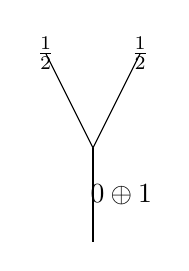
\begin{tikzpicture}[baseline=(current bounding box.center), scale=1.2]
\node at (0,0) {$\frac{1}{2}$};
\node at (1,0) {$\frac{1}{2}$};
\draw (0,0) -- (0.5,-1);
\draw (1,0) -- (0.5,-1);
\draw (0.5,-1) -- (0.5,-2);
\node at (0.8,-1.5) {$0 \oplus 1$};
\end{tikzpicture}
\end{center}

This diagram encodes how two input spin-½ charges combine in the network to yield either a singlet ($j = 0$) or triplet ($j = 1$) excitation.

---

\subsection*{B.2 Clebsch--Gordan Matrix and Contractions}

The Clebsch--Gordan matrix maps product states $\ket{j_1, m_1} \otimes \ket{j_2, m_2}$ to coupled basis states $\ket{J, M}$:

\begin{center}
\begin{tabular}{c|ccc}
Product State & $J=1$ (triplet) & $J=0$ (singlet) \\
\hline
$\ket{+\frac{1}{2}, +\frac{1}{2}}$ & $\ket{1,1}$ & 0 \\
$\ket{+\frac{1}{2}, -\frac{1}{2}}$ & $\frac{1}{\sqrt{2}} \ket{1,0}$ & $\frac{1}{\sqrt{2}} \ket{0,0}$ \\
$\ket{-\frac{1}{2}, +\frac{1}{2}}$ & $\frac{1}{\sqrt{2}} \ket{1,0}$ & $- \frac{1}{\sqrt{2}} \ket{0,0}$ \\
$\ket{-\frac{1}{2}, -\frac{1}{2}}$ & $\ket{1,-1}$ & 0 \\
\end{tabular}
\end{center}

This matrix governs the coefficients used in QGF to construct SU(2)-symmetric tensor blocks. In simulations, each tensor contraction respects this algebra to preserve gauge invariance.

---

\subsection*{B.3 Three-Spin Fusion Chain and Baryon Analogy}

We now examine a chain of three spin-$\frac{1}{2}$ particles:
\[
\left( \frac{1}{2} \otimes \frac{1}{2} \right) \otimes \frac{1}{2} = \frac{1}{2} \oplus \frac{3}{2}
\]

A QGF tensor network that encodes this structure yields a composite excitation in either a total spin-$\frac{3}{2}$ (symmetric baryon-like) or spin-$\frac{1}{2}$ (antisymmetric) configuration.

This mirrors how QCD baryons (e.g., protons, neutrons) arise from combining three spin-$\frac{1}{2}$ quarks. The fusion tree reads:

\begin{center}
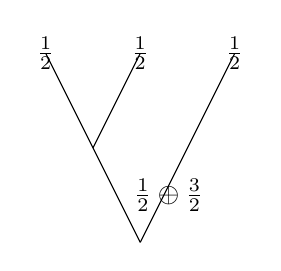
\begin{tikzpicture}[baseline=(current bounding box.center), scale=1.2]
\node at (0,0) {$\frac{1}{2}$};
\node at (1,0) {$\frac{1}{2}$};
\node at (2,0) {$\frac{1}{2}$};
\draw (0,0) -- (0.5,-1);
\draw (1,0) -- (0.5,-1);
\draw (0.5,-1) -- (1.0,-2);
\draw (2,0) -- (1.0,-2);
\node at (1.3,-1.5) {$\frac{1}{2} \oplus \frac{3}{2}$};
\end{tikzpicture}
\end{center}

---

\subsection*{B.4 Simulation Note (Libraries)}

To simulate these dynamics numerically, one can enforce SU(2) fusion via block-diagonal tensor formats using:

\begin{itemize}
  \item \texttt{ITensor} (Julia/C++) — supports symmetric tensors.
  \item \texttt{quimb} (Python) — for numerical contraction.
  \item \texttt{symtensor} — for block-structured tensor networks.
\end{itemize}

These platforms ensure contraction paths follow Clebsch–Gordan logic, preserving fusion rules numerically.

---

\textbf{Conclusion:} QGF encodes gauge symmetry and matter coupling via categorical fusion rules. The SU(2) example illustrates how spin composition, tensor structure, and gauge interaction all emerge algebraically within the entanglement network.



\bibliographystyle{unsrt}
\bibliography{references}

\vspace{1cm}
\noindent\textit{This version is archived at \href{https://doi.org/10.5281/zenodo.15384837}{doi.org/10.5281/zenodo.15384837} to establish public authorship and timestamp.}


\end{document}
